\documentclass[a4paper,11pt]{article}
\usepackage{amsmath,amsthm,amsfonts,amssymb,amscd,amstext,vmargin,graphics,graphicx,tabularx,multicol} 
\usepackage[francais]{babel}
\usepackage[utf8]{inputenc}  
\usepackage[T1]{fontenc} 
\usepackage{pstricks-add,tikz,tkz-tab,variations}
\usepackage[autolanguage,np]{numprint} 

\setmarginsrb{1.5cm}{0.5cm}{1cm}{0.5cm}{0cm}{0cm}{0cm}{0cm} %Gauche, haut, droite, haut
\newcounter{numexo}
\newcommand{\exo}[1]{\stepcounter{numexo}\noindent{\bf Exercice~\thenumexo} : \marginpar{\hfill /#1}}
\reversemarginpar


\newcounter{enumtabi}
\newcounter{enumtaba}
\newcommand{\q}{\stepcounter{enumtabi} \theenumtabi.  }
\newcommand{\qa}{\stepcounter{enumtaba} (\alph{enumtaba}) }
\newcommand{\initq}{\setcounter{enumtabi}{0}}
\newcommand{\initqa}{\setcounter{enumtaba}{0}}

\newcommand{\be}{\begin{enumerate}}
\newcommand{\ee}{\end{enumerate}}
\newcommand{\bi}{\begin{itemize}}
\newcommand{\ei}{\end{itemize}}
\newcommand{\bp}{\begin{pspicture*}}
\newcommand{\ep}{\end{pspicture*}}
\newcommand{\bt}{\begin{tabular}}
\newcommand{\et}{\end{tabular}}
\renewcommand{\tabularxcolumn}[1]{>{\centering}m{#1}} %(colonne m{} centrée, au lieu de p par défault) 
\newcommand{\tnl}{\tabularnewline}

\newcommand{\bmul}[1]{\begin{multicols}{#1}}
\newcommand{\emul}{\end{multicols}}

\newcommand{\trait}{\noindent \rule{\linewidth}{0.2mm}}
\newcommand{\hs}[1]{\hspace{#1}}
\newcommand{\vs}[1]{\vspace{#1}}

\newcommand{\N}{\mathbb{N}}
\newcommand{\Z}{\mathbb{Z}}
\newcommand{\R}{\mathbb{R}}
\newcommand{\C}{\mathbb{C}}
\newcommand{\Dcal}{\mathcal{D}}
\newcommand{\Ccal}{\mathcal{C}}
\newcommand{\mc}{\mathcal}

\newcommand{\vect}[1]{\overrightarrow{#1}}
\newcommand{\ds}{\displaystyle}
\newcommand{\eq}{\quad \Leftrightarrow \quad}
\newcommand{\vecti}{\vec{\imath}}
\newcommand{\vectj}{\vec{\jmath}}
\newcommand{\Oij}{(O;\vec{\imath}, \vec{\jmath})}
\newcommand{\OIJ}{(O;I,J)}


\newcommand{\reponse}[1][1]{%
\multido{}{#1}{\makebox[\linewidth]{\rule[0pt]{0pt}{20pt}\dotfill}
}}

\newcommand{\titre}[5] 
% #1: titre #2: haut gauche #3: bas gauche #4: haut droite #5: bas droite
{
\noindent #2 \hfill #4 \\
#3 \hfill #5

\vspace{-1.6cm}

\begin{center}\rule{6cm}{0.5mm}\end{center}
\vspace{0.2cm}
\begin{center}{\large{\textbf{#1}}}\end{center}
\begin{center}\rule{6cm}{0.5mm}\end{center}
}



\begin{document}
\pagestyle{empty}
\titre{Interrogation: Soustractions et cercles }{Nom :}{Prénom :}{Classe}{Date}


\exo{3} Compléter le texte suivant :


\bmul{2}

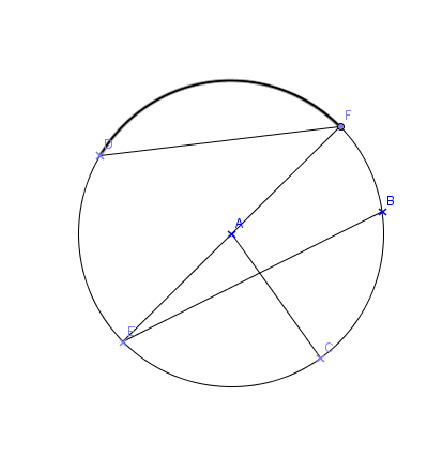
\includegraphics[scale=1]{cercle.eps} 

\columnbreak

\bi
\item Le ....................... $(C)$ de .......................... A passe par les points F, B, D, C et E.\\

\item Les segments [AF], [AC] et .............. sont des  ................. du cercle $(C)$.\\

\item Le segment [FE] est un ........................... du cercle $(C)$.\\

\item $\overset{\displaystyle\frown}{DF}$ est .......................................................
\ei




\emul


\exo{2} Poser et effectuer les opérations suivantes :               \\

\bmul{2}

213,9 - 86,23

\vspace*{5cm}

\columnbreak

549,72 – 453,8
\vspace*{5cm}

\emul


\exo{1} Entourer en bleu, pour chaque calcul, le meilleur ordre de grandeur :\\

\begin{tabular}{|c|c|c|c|c|}
\hline 
143,2 – 98,7 & 40 & 45 & 50 & 245 \\ 
\hline 
345,56 - 129,56 & 200 & 480 & 210 &  230 \\ 
\hline 
\end{tabular} 

\vspace*{1cm}

\exo{1,5} Pour chaque problème, indiquer l'opération à effectuer pour le résoudre et écrire le résultat.

\begin{flushleft}
\includegraphics[scale=1]{tabsoust.eps}  
\end{flushleft}

\newpage

\exo{2,5}

\initq 
\q Pour tapisser sa chambre, Antoine achète 4 rouleaux de papier peint au prix total de 18,40 euros. N'ayant qu'un billet de 20 euros, il lui manque 2,11 euros pour acheter la colle. Quel est le prix de la colle ?\\

\reponse[5]\\


\q La voiture de Stéphane consomme 5 litres d'essence pour 100 km parcourus. Il fait le plein du réservoir ; il dispose alors de 50 L. Il effectue un déplacement de 495 km, puis le week-end il effectue un trajet de 295 km. Le lundi suivant, pour son travail, il doit se rendre à 155 km de chez lui.\\

En utilisant des ordres de grandeurs, déterminer si Stéphane peut aller faire l'aller-retour du lundi sans s'arrêter dans une station service.\\

\reponse[6]









\end{document}
